%!TEX root = ../report.tex
\chapter{Calibration} % (fold)
\label{cha:calibration}

\section{Camera calibration} % (fold)
\label{sec:camera_calibration}
As stated in \ref{sec:cam_calib}, a calibration for the stereovision rig needs to be performed to solve the camera model.
To do so, a predefined ROS node has been applied since it minimizes the user interaction and simplifies the process. 
The node only needs to be provided enough images of a 2D calibration pattern in different positions since it implements the calibration technique presented in \cite{Zhang}. 
The calibration pattern used is a laser-printed chessboard. 
During the acquisition of the images, it has been tried to provide the wider possible range of positions and orientations of the pattern in the images in order to supply the maximum and more varied set of points to the algorithm.
Once the homography between the image plane and the pattern is solved, the more varied the set of projected points is, the better is the estimation of the projection matrix obtained through projection error minimization, as described in \cite{Hartley}. 

Once the process is over, the outputs of the node are the camera and projection matrices of the two cameras, the set of parameters for the distortion model and the homography matrix for the image rectification (see figure \ref{fig:undistorsion}).
Since the projection matrices will be used for the computation of the fundamental matrix during the triangulation calculus, their quality will heavily influence the overall performance of the system. 
Therefore, a special commitment has been applied to this step. 

	\begin{figure}[!ht]
		\centering
		\begin{subfigure}{.49\textwidth}
		  \centering
		  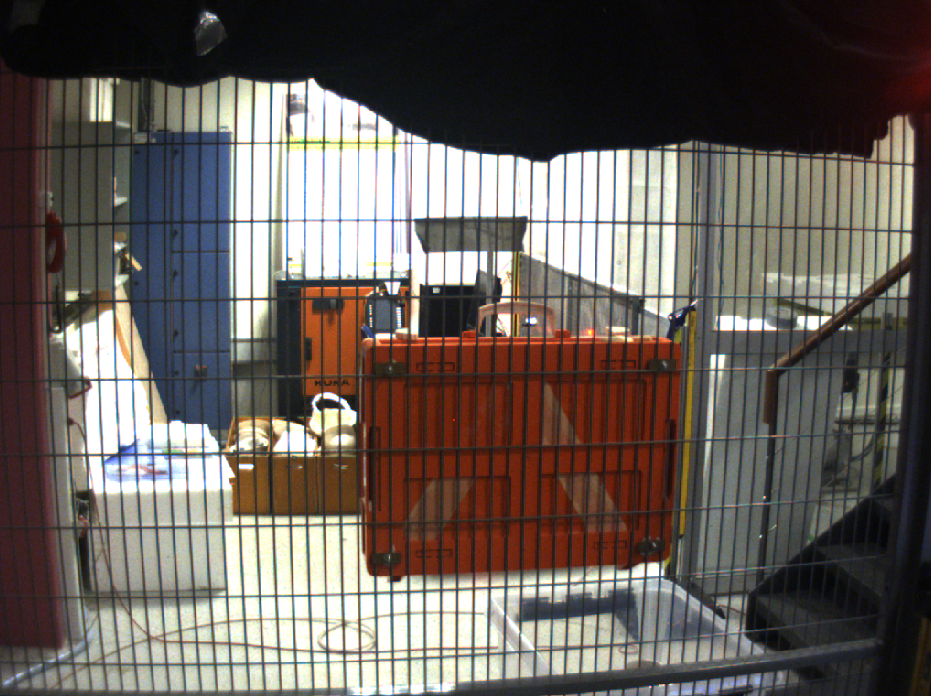
\includegraphics[width=0.95\textwidth]{figures/distorted}
		\end{subfigure}%
		\begin{subfigure}{.49\textwidth}
		  \centering
		  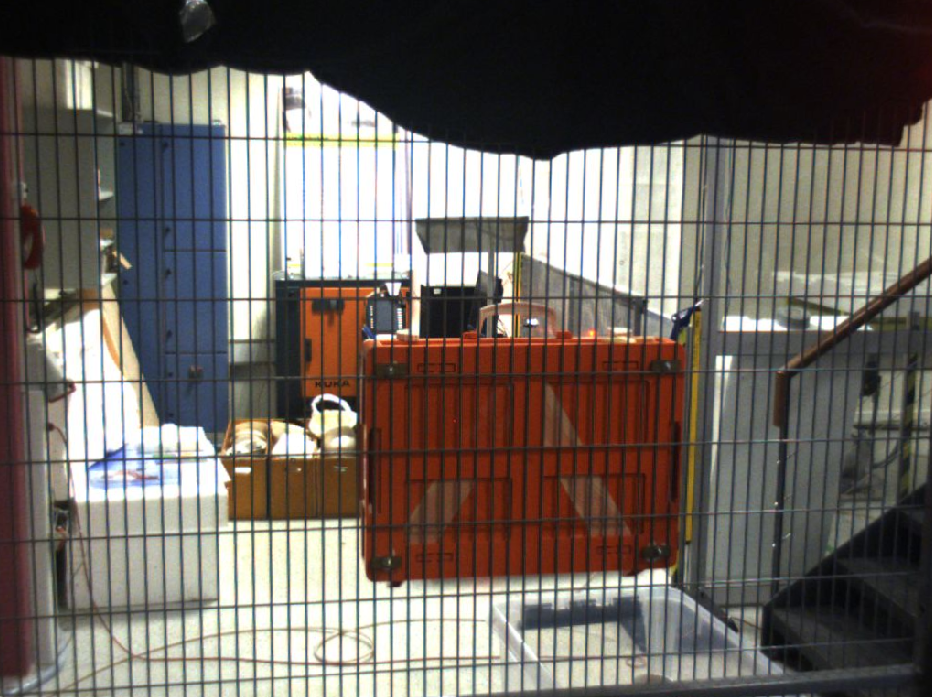
\includegraphics[width=0.95\textwidth]{figures/undistorted}
		\end{subfigure}
		\caption{Image before and after apply undistortion}
		\label{fig:undistorsion}
	\end{figure}

% section camera_calibration (end)

\section{Robot calibration} % (fold)
\label{sec:robot_calibration}
The calibration of the robot has not been carried out. The reasons that support this decision are:
\begin{enumerate}
	\item For the \textbf{extrinsic calibration}, the calibration with the camera in the tool mount could have been implemented. But the lack of real and precise measurements mechanisms that would led to real calibration data, haven't been found. If founded, the experiment would have been to place a reference object with in a known position and then calculate its theoretical position based on the information from the cameras and the robot's configuration.
	\item In the case of the \textbf{intrinsic calibration}, the same reasons are given. No valid measurements tools were found for the measurements of the link's length, angles and poses in the work cell. However, if this tools were available, the process would be to measure the link's length to create a Denavit Hartenberg forward kinematics model so the measurements would have been treated easily. Sending the robot to an specified Q, the difference between the real configuration and the desired one would have lead to a model of intrinsic calibration.
\end{enumerate}

Despite the robot's calibration has not been carried out, a plot (see figure TODO) with the error between the desired configuration and the real one is shown. As it can be seen, the error is not in the order of affect determinately to our project.
% section robot_calibration (end)

% chapter calibration (end)